\documentclass[11pt]{article}
\usepackage[utf8]{inputenc}
\usepackage[T1]{fontenc}
\usepackage[margin=1in]{geometry}
\usepackage{float}
\usepackage{
    mathtools,
    amssymb,
    amsthm,
    units,
    hyperref,
    graphicx,
    fancyhdr,
    authblk,
    natbib,
    multicol,
    enumitem,
    caption,
    subcaption,
    float,
    bbm
}

\usepackage{booktabs}

%\usepackage[style=authoryear, backend=biber]{biblatex}
%\addbibresource{references.bib}

% Force footnotes to be at the bottom of the page
\usepackage[bottom]{footmisc}

\captionsetup{font={footnotesize, sf}, labelfont=bf}

\setlength\parindent{0.2pt}
\setlength{\parskip}{1em}

\usepackage{lipsum}

%\setlength\parindent{0.2pt}
%\setlength{\parskip}{1em}

% Allow arrays of equations to span several pages
\allowdisplaybreaks

\hypersetup{
    colorlinks = true, 
    urlcolor   = blue, 
    linkcolor  = blue, 
    citecolor  = red   
}

\cfoot{\thepage}
\setlength{\headheight}{15pt}

\renewcommand\Authfont{\bfseries\normalsize}
\renewcommand\Affilfont{\small\normalfont}

\author[1]{Ziang Gao}
\author[1]{Adam Hetherwick}
\author[1]{Danny Kuei}
\author[1]{Cody Vig}

\affil[1]{%
    \centering
    \emph{Department of Statistics, University of California, Davis.}\protect\\
    \texttt{\{zggao, ajhetherwick, dkuei, cvig\}@ucdavis.edu}
}

\title{%
    On the Class Size Trend Effect on Student Performance in Early Childhood Education\footnote{The code used to generate the data in this report can be found here: \href{https://github.com/ucd-sta-207-project/ucd-sta-207-project}{https://github.com/ucd-sta-207-project/ucd-sta-207-project}}
}

\date{March 16, 2026}

%%% --------------------------- Begin Document --------------------------- %%%
\begin{document}

\maketitle

\begin{abstract}

An analysis was performed on the dataset generated from the Project STAR (\emph{Student to Teacher Achievement Ratio}) experiment conducted on Tennessee elementary schools in the late 1980's. Our analysis seeks to validate some of the significant findings brought to light by past research. Our work corroborates the existing literature by showing that students in smaller class sizes produce statistically significantly better kindergarten mathematics SAT scores when compared to students in larger classes, especially for students from disadvantaged backgrounds. We also expand upon the claims made by other researchers that small class sizes lead to diminishing achievement gains over time by examining third-grade mathematics SAT scores among students who did not comply with their assigned class size. We find that neither the small-to-large class cohort nor the large-to-small class cohort see significantly better scores that those who stayed in large classes all four years.

\end{abstract}


%%% ----------------------------- Background ----------------------------- %%%
\section{Background}\par
\label{section:background}
%%% DONE: Cody to write

\subsection{Project STAR}
Project STAR (\emph{Student to Teacher Achievement Ratio}) was a large-scale, longitudinal, randomized experiment conducted between 1985 and 1989 and examined the effect of class size on student performance in students' early childhood education (kindergarten and early elementary school). All schools were invited to participate and were required to have at least one of the following class sizes: small (containing 13 to 17 students), regular (containing 22 to 26 students), or regular with a full-time teacher's aid.

The project was managed by the Tennessee State Department of Education and the research was advised and operationally supported by researchers at four neighboring universities: Memphis State University, Tennessee State University, the University of Tennessee at Knoxville, and Vanderbilt University. Though the ideal would have been a perfectly random assignment of class sizes to instructors and students to class sizes, not all schools agreed to or were capable of being part of the study, so concessions were made. The project required participating schools to accept the random assignment of teachers and students to different class types, and all teachers had to be certified for their grade level. Although about 180 schools initially expressed interest, only those with sufficient kindergarten enrollment (at least 57 students) could participate because the study used a within-school experimental design.

Ultimately, 79 schools across 42 school systems were selected to ensure representation across districts, school types, and regions. In the 1986 academic year, the project included roughly 300 classes: 128 small classes (about 1,900 students), 101 regular classes (about 2,300 students), and 99 regular classes with teacher aides (about 2,200 students) \cite{achilles2008star}.

\subsection{Literature Review}
Large scale randomized experiments are rare in the education sector. As such, this project has been studied extensively and much insight has been gained from it. Research on class-size reduction has developed substantially over the past several decades, and much of the evidence comes from Project STAR. A large body of literature has used this dataset to evaluate both the short-term and long-term consequences of early exposure to smaller classes, particularly for disadvantaged students.

Early research emphasizes the positive academic effects of smaller classes in early grades. Jeremy D. Finn (1998) \cite{finn1998_class_size_students_risk} reviewed the existing literature on class-size reduction and focused particularly on results emerging from Project STAR. The review concludes that smaller classes are associated with higher academic achievement in early elementary school. The benefits appear to be strongest for students considered academically \emph{at risk}, including those from low-income backgrounds and historically disadvantaged groups. Finn notes that smaller classes may lead to greater student engagement, participation, and effort in the classroom, which he proposed as potential mechanisms through which reduced class size contributes to improved learning outcomes. Finn went on to state several open questions in the literature, including whether these early gains persist over time and how multiple years of exposure to small classes influence longer-term academic trajectories.

Subsequent research has addressed these questions by examining the long-term consequences of early class-size reductions. Using longitudinal data from Project STAR, Jeremy D. Finn et al. (2005) \cite{finn2005_small_classes_graduation} tracked nearly 5,000 students from kindergarten through high school to evaluate whether early class size affects the likelihood of graduating from high school. Their findings suggest that sustained exposure to small classes in the early grades has significant long-term benefits. Students who spent three or more years in small classes were statistically significantly more likely to graduate than their peers in larger classes. Four years of exposure to small class sizes was associated with an increase of approximately 11.5 percentage points in high school graduation rates. Effects were demonstrated to be particularly pronounced for students from low-income backgrounds. The authors also find that early academic achievement is strongly correlated with eventual graduation, which suggests that the short-term gains observed in smaller classes may contribute to improved long-term educational attainment.

Diane Whitmore Schanzenbach (2007) \cite{schanzenbach2007_project_star} surveyed the existing literature generated by the experiment and concluded that it provided credible experimental evidence on the effects of class-size reduction. Across numerous studies, the evidence universally indicates that smaller classes in the early grades lead to statistically significant improvements in student achievement. She further corroborated that the largest benefits appear among disadvantaged students (i.e., those from low-income and minority backgrounds). The author also noted that students who begin in small classes in kindergarten and remain in them for multiple years experience the largest gains, albeit with some diminishing returns in the achievement improvements.

To summarize, the surrounding literature suggests that class-size reduction in the early elementary grades produces statistically significant academic benefits across various socioeconomic and demographic variables, especially among at-risk students. The evidence from Project STAR demonstrates both short-term improvements in student achievement and long-term gains in educational attainment, including higher high school graduation rates. 


%%% ------------------------ Question of Interest ------------------------ %%%
\section{Question of Interest}\par
\label{section:question}
%%% DONE: Cody to write
We see from Section \ref{section:background} that it is well-understood based on the existing literature that smaller class sizes yield statistically significantly higher student achievement, both in the short-term and in the long-term. Of particular interest to us is the remark by Schanzenbach \cite{schanzenbach2007_project_star} that the small-class cohort sees diminishing returns in achievement gains in later years.  We had hoped to expand upon the existing literature by examining attrition among the small class cohort to see if most of the achievement gain was retained among the students who left the small class pipeline early. Unfortunately, as we will see in Section \ref{section:descriptive}, attrition from the small class cohort was uncommon, i.e., most students who started in small classes stayed in small classes for the remainder of the study. Although there is a nontrivial number of students who did leave small classes in favor of regular ones, the sample size is small enough to risk substantial bias.

During this analysis, it was observed that attrition from the large class cohort to the small class cohort was much more common. This could be due to parental intervention, in which some parents request that their children not be disadvantaged by being placed in larger classrooms and be placed in the smaller one in the next year. Nonetheless, this large attrition rate allows us to ask a similar question about the potential achievement gains among students who joined the small class cohort late.

As such, our analysis is twofold: corroborate the existing literature and expand upon it by address attrition. To do this, we address the following questions:

\begin{enumerate}
    \item Do smaller class sizes disproportionately benefit low-income students in early elementary school?
    \item For students who begin their academic journey in regularly sized classrooms, is it educationally advantageous to switch to smaller classes in later years?
\end{enumerate}

In each case, we measure the student's academic performance by their grades on the mathematics portion of the Stanford Achievement Test (SAT).

Answers to these questions have significant implications on data-driven educational policies and procedures. For instance, the analysis does to address question 2 could help inform intervention strategies for struggling students in later years. These results may also alleviate budgeting concerns associated with the implementation of smaller classrooms school-wide. If it turns out to be advantageous to switch to a smaller classroom later in a student's educational journey, it may be wise to offer smaller classrooms at certain grade levels. Analogously, if returns in achievement gains diminish in later years among students whose educational journey is exclusively in small classrooms, then it might be financially beneficial to offer smaller class sizes only in the earliest grade levels.

%%% ------------------------ Descriptive Analysis ------------------------ %%%
\section{Descriptive Analysis}\par
\label{section:descriptive}
\subsection{Overview}
Before conducting a formal statistical analysis, we first explore the structure and key characteristics of the dataset through exploratory data analysis. The purpose of this section is to understand the distribution of school characteristics, student demographics, socioeconomic status, and academic results. 
\subsection{School Characteristics}
We begin by examining the distribution of school environments.
Figure \ref{fig:urbanicity} shows the distribution of school urbanicity in the dataset. The majority of schools are located in rural areas, followed by suburban and inner-city schools, while only a small proportion are classified as urban.

This variation in school location suggests that students in the dataset are given different educational context due to the location of schools, because the school environment may influence the available resources and learning conditions. So, school urbanicity is included as one of the explanatory factors in our ANOVA model.

\begin{figure}[H]
\centering
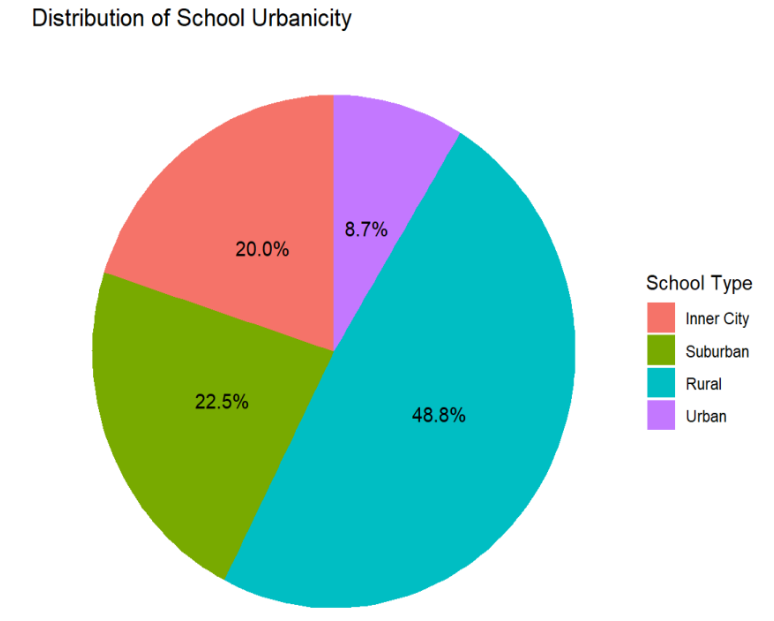
\includegraphics[width=0.5\textwidth]{urbanicity.png}
\caption{Distribution of School Urbanicity}
\label{fig:urbanicity}
\end{figure}

\subsection{Student Demographics}
Next, we examine the demographic composition of students. As shown in Figure \ref{fig:race}, the racial distribution indicates that White students represent the largest portion of the sample, followed by Black students, while other racial groups account for a relatively small share of observations.

%%% Removed for clarity
%Due to the limited sample sizes of other race groups, they are combined into a single “Other” category for the further analysis.

Due to the limited sample sizes of the other race groups, including them in the subsequent analysis would generate potentially substantial bias. As such, racial groups other than White and Black were removed from the dataset before conducting any statistical inference.

These demographic characteristics are relevant because differences in student background can be associated with variation in academic performance. Therefore, race and gender are included as explanatory variables in the mixed effects model.
\begin{figure}[H]
\centering
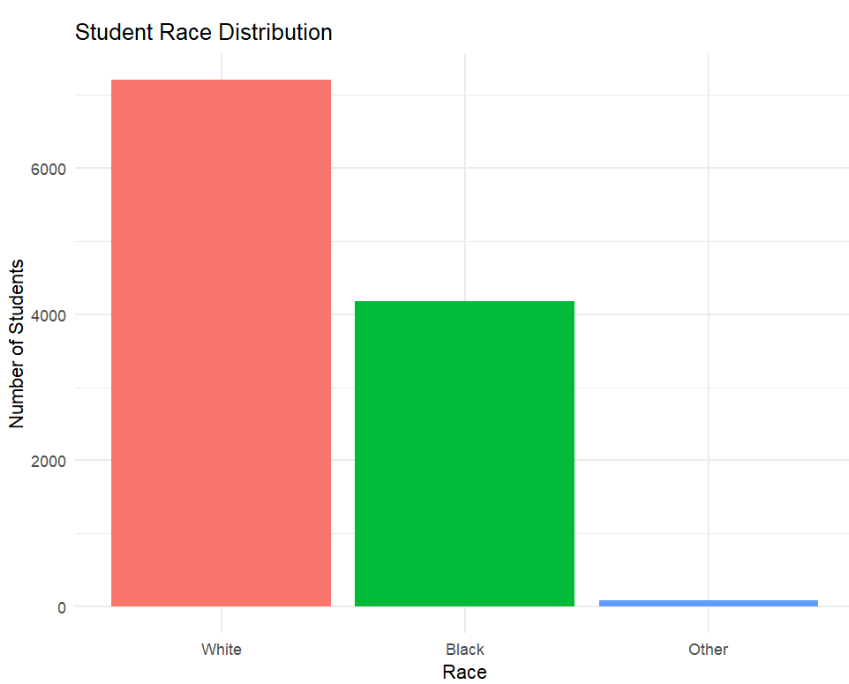
\includegraphics[width=0.5\textwidth]{race.png}
\caption{Distribution of Student Race}
\label{fig:race}
\end{figure}

\subsection{Socioeconomic Status}
Socioeconomic status (SES) is measured using the percentage of students receiving free or reduced-price lunch. Schools with higher percentages of students receiving free lunch are considered to have lower socioeconomic status.

The histogram of free lunch percentages (Figure \ref{fig:freelunch}) shows substantial variation in SES across schools. Many schools fall within the middle SES range, while a considerable number belong to lower SES categories. For visualization purposes in the EDA, we categorize schools into SES groups based on the free lunch percentage. However, in the subsequent analysis, we use the continuous free lunch percentage variable as the key explanatory variable in both the ANOVA model and the mixed-effects model.
\begin{figure}[H]
\centering
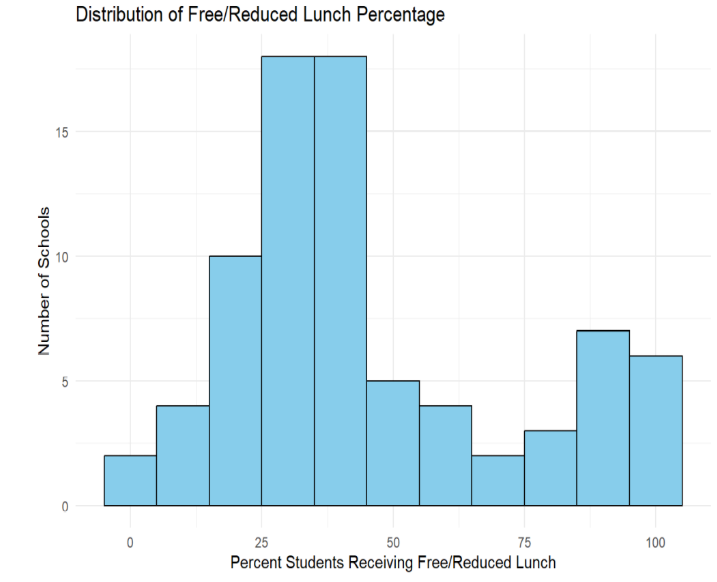
\includegraphics[width=0.5\textwidth]{lunch.png}
\caption{Distribution of Student receivng free lunch}
\label{fig:freelunch}
\end{figure}
\subsection{Student Test Score Distributions}
Next, we examine the distribution of student academic outcomes. Boxplots of math and reading scores across grades and gender reveal several patterns.

Consider Figure \ref{fig:math_reading_scores}. First, average test scores increase as students progress from kindergarten to grade three, reflecting expected academic development over time. Second, the distributions of scores for male and female students appear relatively similar across grades. These patterns provide an initial overview of the data and help us understand the distribution of outcomes before we move on to more formal statistical analysis examining the effects of class
size.

\begin{figure}[H]
\centering

\begin{subfigure}{0.49\textwidth}
    \centering
    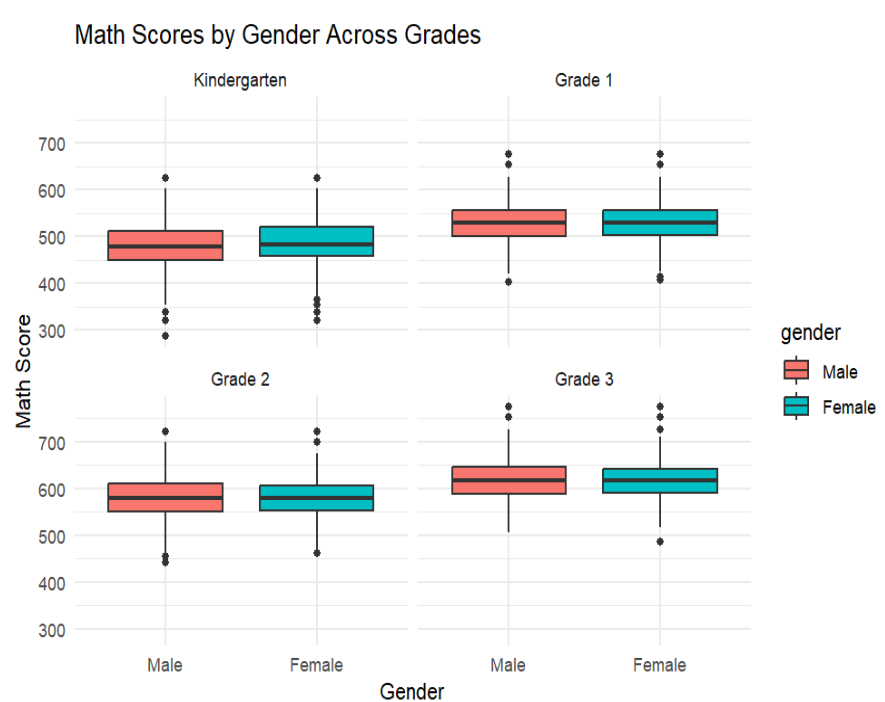
\includegraphics[width=\linewidth]{math.png}
    \caption{Math Scores Across Grade}
    \label{fig:math}
\end{subfigure}
\hfill
\begin{subfigure}{0.49\textwidth}
    \centering
    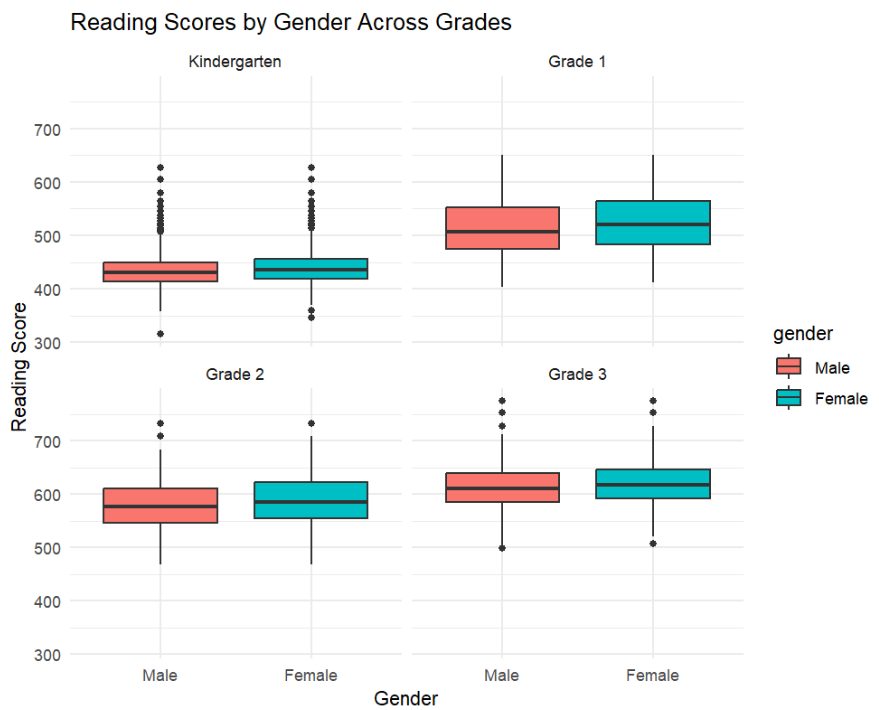
\includegraphics[width=\linewidth]{reading.png}
    \caption{Reading Scores Across Grade}
    \label{fig:reading}
\end{subfigure}

\caption{Test Scores Across Grades}
\label{fig:math_reading_scores}
\end{figure}

Figures \ref{fig:math} and \ref{fig:reading} show the similarity between reading and math test scores. We notice that all grades display relatively similar relationships to each other and distributions among students. We also notice that the scaled test scores increase for both math and reading as students advance to higher grades. This coincides with the information stated in the Project STAR Summary Report (page 19) that math and reading effects are similar \cite{glass_1984}. Therefore, math scores alone are a sufficient performance metric for students' academic achievements. 

\subsection{Non-Compliance}

Figure \ref{fig:sankey} shows the pipeline students who persisted through all four years of the experiment took. Note that students who did not participate in all four years of the experiment (e.g., those that transferred to a different, non-participating school before completing the third grade) have been removed from the diagram and from the analysis altogether. Additionally, for the present analysis we ignored all students who took classes in regularly sized classrooms with a full-time teacher's aid. This decision was made to isolate the small class size effect and to eliminate the additional variance that would be generated by combining the two regular class size groups. 

\begin{figure}[H]
    \centering
    
\includegraphics[width=0.95\textwidth]{img/sankey_classtype.png}
    \caption{Attrition and throughput among students who persisted in the experiment through all four years. Those that transferred out of the system early or joined late have been removed. Students in regularly sized classes with a full-time teacher's aid have also been removed.}
    \label{fig:sankey}
\end{figure}

It is apparent that the significant majority of students who started on a particular path, stayed on that path for the remainder of the experiment. It is also apparent that the small class size cohort was substantially larger than the regular class size cohort. Finally, noncompliance is present, but it is comparatively small. Of interest, most students who did not comply with their class size allocation switched from large class sizes to smaller ones. This could be due to more academically conscious parents advocating for their children to be given the best possible treatment, or potentially due to counselor recommendation for students who were struggling in regularly sized classrooms. Attrition from small class sizes to larger ones is almost completely negligible, especially after the Kindergarten to Grade 1 transition.

\subsection{Summary}

Overall, the exploratory analysis highlights meaningful variation in school environment, socioeconomic status, and student performance. These patterns motivate the modeling strategy used in the next section, where we estimate the effects of class size, free lunch status, and school urbanicity using a three-factor ANOVA model, and further examine student-level trends using a mixed effects model.

%%% TODO: Cody to add sankey diagram and discussion

%%% ------------------------ Inferential Analysis ------------------------ %%%
\section{Inferential Analysis}\par
\label{section:inferential}
%%% TODO: Danny and Adam to write

\subsection{Three Way ANOVA Model}

To evaluate the relationship between small class size and socioeconomic status, we initially  fit a preliminary fixed ANOVA model \ref{eqn:model1} with kindergarten math scores as the outcome. Free lunch status was used a proxy for socioeconomic status while school urbanicity was used to capture the effects of school differences. To determine if small class size disproportionately benefit low-income students in early elementary school interaction terms were additionally fit between class size and free lunch and compared to the additive model using the extra sum of squares of $F$-test (Table \ref{tab:ftest}). The results indicate that  the interaction model did not provide a significant better fit than the additive model ($p = 0.880$), suggesting the effect of class size does not vary significant by socioeconomic status. 

%%% Danny, please feel free to change this, but please keep the `\label{}` so I can reference this in later sections.
\begin{equation}
    \label{eqn:model1}
    Y_{ijkl} = \mu + \alpha_i + \beta_j + \gamma_k + \varepsilon_{ijkl}
    \quad ; \quad \varepsilon_{ijkl} \; \overset{iid}{\sim} \; N(0, \sigma^2) \
\end{equation}

where:
\begin{itemize}[nosep]
\item $Y_{ijkl}$ is the kindergarten math score of the $l$-th student in the $k$-th urbanicity category, the $j$-th free lunch status, and $i$-th class type. 
\item $\alpha_i$ is the main effect of class size
\item $\beta_j$ is the main effect of free lunch
\item $\gamma_k$ is the main effect of urbanicity
\item $\varepsilon_{ijkl}$ is the random error term
\end{itemize}



\begin{table}[htbp]
\centering
\caption{Comparison of Three-way ANOVA Candidate Models by F-test}
\label{tab:ftest}
\begin{tabular}{lccccc  c}
\toprule
\textbf{Model} & \textbf{Parameters} & \textbf{Residual df} & \textbf{RSS} & \textbf{Sum Sq.} & \textbf{F-stat} & \textbf{p-value} \\
\midrule
Additive & 8 & 1336 & 2619558 & & & \\ 
Interaction \\ (class size $\times$ free lunch) & 9 & 1335 & 2619513 & 44.9 & 0.023 & 0.880 \\
\bottomrule
\end{tabular}
\end{table}

The results as shown in Table \ref{tab:fixed_anova_results} indicate that class type ($p = 1.41 \times 10^{-5}$) and non-free lunch ($p = 4.47 \times 10^{-12}$) have a statistically significant impact on math scores. Class type had a $F$-value of 18.993, well above the critical threshold of 3.85, meaning that the differences between small and regular class types are likely not due to random chance. Non-free lunch was even more influential with an $F$-value of 48.790, indicating socioeconomic status is a strong predictor of math scores. Urbanicity was not found to be a significant factor ($p = 0.74$).  

While the main effects of class type and free lunch are significant, the $F$-test showing that the interaction term was not significant suggests that small class size does not disproportionately benefit low-income students. Furthermore, the substantial residuals sum of squares (2,619,558) indicates a significant portion of the variance in math scores remains unexplained by these factors alone, justifying a move towards more complex modeling. 


\begin{table}[htbp]
\centering
\caption{ANOVA Table for Three Factor Model}
\label{tab:fixed_anova_results}
\begin{tabular}{lcccccc}
\toprule
\textbf{Variable} & \textbf{df} & \textbf{Sum Sq.} & \textbf{Mean Sq.} & \textbf{F-value} & \textbf{F-critical} & \textbf{p-value} \\
\midrule
Class Type & 1 & 37239.930 & 37239.930 & 18.993 & 3.85 & 1.41e-05 \\
NonFree Lunch & 1 & 95665.547 & 95665.547 & 48.790 & 3.85 & 4.47e-12 \\
Urbanicity & 3 & 2456.925 & 818.975 & 0.418 & 2.61 & 0.74 \\
Residuals & 1336 & 2619558.218 & 1960.747 &  &  & \\
\bottomrule
\end{tabular}
\end{table}

\subsection{Mixed Effects Model}
%%% DONE: Danny to write

Next, to explore if it was educationally advantageous to switch to smaller class in later years, we created a trend variable where we looked at if students switched class size between kindergarten and 3rd grade. This creates four factor groups which are constant regular, constant small, regular to small, and small to regular class size in which the former two were compliers and the ladder two were non-compliers. To examine the effect of the trend variable while controlling for additional covariates, we fit a more complex mixed effects model with random intercept for school and 3rd grade math scores as the outcome (Equation \eqref{eqn:model2}). A random intercept for school was included because we wanted to generalize the results of our model to the population outside of STAR. This allows the baseline math score to vary across schools. Furthermore, while urbanicity may capture some school-level differences, we expect there may be unexplained variation that is not captured by this variable. In addition to the free lunch variable from the previous model, other variables of interest included demographic variables such as gender and race as well as teacher years of experience. 

\begin{equation}
    \label{eqn:model2}
    Y_{ij} = \beta_0
        + \beta_1 \cdot \mathbbm{1}_{\mathrm{trend}}
        + \beta_2 \cdot \mathbbm{1}_{\mathrm{gender}}
        + \beta_3 \cdot \mathbbm{1}_{\mathrm{race}}
        + \beta_4 \cdot \mathbbm{1}_{\mathrm{freelunch}}
        + \beta_5 \cdot \mathbbm{1}_{\mathrm{tyears}}
        + b_{0,j} + \varepsilon_{ij},
\end{equation}
where $b_{0,j} \sim N(0, \sigma_b^2)$, $\varepsilon_{ij} \sim N(0, \sigma^2)$, and $\mathbbm{1}_{S} \equiv \mathbbm{1}_{S}(X)$ is the indicator function for $X \in S$.

Similar to the Three Way ANOVA Model, interactions were initially fit in which BIC scores and the Likelihood Ratio Test (LRT) were used to find significance (Table \ref{tab:lrt}). Although both interactions interactions had a lower -2log-Likelihood suggesting better fit, the results from the BIC and the LRT p-value suggest that the additive model is sufficient. Thus, our final mixed effects model is the additive model as shown in Equation \eqref{eqn:model2}. 

\begin{table}[htbp]
\centering
\caption{Comparison of Mixed Effects Candidate Models by Likelihood Ratio Test}
\label{tab:lrt}
\begin{tabular}{lcccccc}
\toprule
\textbf{Model} & \textbf{Parameters} & \textbf{AIC} & \textbf{BIC} & \textbf{-2log(L)} & \textbf{Chi-sq} & \textbf{p-value} \\
\midrule
Additive & 10 & 12928 & 12980 & 12908 & & \\ 
Interaction (trend $\times$ freelunch) & 13 & 12927 & 12994 & 12901 & 7.719 & 0.052 \\
Interaction (trend $\times$ race & 12980 & 13 & 12999 & 12906 & 2.104 & 0.551 \\
\bottomrule
\end{tabular}
\end{table}


The results of our mixed effects model (Table \ref{tab:mixed_results}) suggest that the trend effect was statistically significant only for the complier group ($p = 0.019$). Holding all other variables constant, we see that student who were in constant small class size scored on average 5.6 higher in math compared to those in constant regular class size. Both groups that switched class size also saw increases in scores, but the p-values were insignificant ($p = 0.338$, $p = 0.055$). This means we have insufficient evidence to conclude that switching class size is advantageous.

Other significant covariates included race ($p = 1.22 \times 10^{-4}$) and free lunch status ($p = 1.04 \times 10^{-11}$). We found that on average, Black students scored around 13.4 points lower than White students suggesting disparities in educational outcomes across racial groups. However, the most significant factor was socioeconomic status, with student who did not receive free lunch performing 16.6 points better than those who received free lunch. Gender and teacher years of experience did not have a significant effect according to the model.

\begin{table}[htbp]
\centering
\caption{Results of Mixed Effects Additive Model}
\label{tab:mixed_results}
\begin{tabular}{lccccc}
\toprule
\textbf{Variable} & \textbf{Estimate} & \textbf{Standard Error} & \textbf{df} & \textbf{t-statistic} & \textbf{p-value} \\
\midrule
Intercept & 615.928 & 3.922 & 485.138 & 157.051 & <2e-16 \\ 
trendConstantSmall & 5.636 & 2.399 & 1263.158 & 2.349 & 0.019 \\
trendRegtoSmall & 3.577 & 3.731 & 1280.929 & 0.959 & 0.338 \\
trendSmalltoReg & 13.871 & 7.214 & 1204.866 & 1.923 & 0.055 \\
genderFemale & -1.120 & 1.986 & 1232.092 & -0.564 & 0.563 \\
raceBlack & -13.443 & 3.463 & 383.702 & -3.882 & < 1.22e-4 \\
NonFree Lunch & 16.551 & 2.411 & 1279.918 & 6.865 & < 1.04e-11 \\
Teacher Years & 0.212 & 0.133 & 1171.730 & 1.589 & 0.112 \\
\bottomrule
\end{tabular}
\end{table}

For the random intercept, we examined the variances and standard deviations for the school random effects (between-school variation) and the residuals (within-group variation among students) as shown in Table \ref{tab:mixed_intercept_results}. The Intraclass Correlation Coefficient (ICC) was used to quantify the proportion of variance attributed to difference between schools \eqref{eqn:icc}. With an ICC of 0.1356, we see that around 13.6\% of the variation in scores is due to school differences. While this suggests most of the variation is attributed to between students within schools rather than between schools, the results is still substantial and consistent with findings in educational studies \cite{shear2026_icc}.

\begin{equation}
    \label{eqn:icc}
    \begin{aligned}
    \rho &= \frac{\sigma^2_\alpha}{\sigma^2_\alpha + \sigma^2}  \\
    &= \frac{192.2}{192.2 + 1224.7} \\
    &= 0.1356
    \end{aligned}
\end{equation}

\begin{table}[htbp]
\centering
\caption{Results of Mixed Effects Additive Model (Random Variable)}
\label{tab:mixed_intercept_results}
\begin{tabular}{lcc}
\toprule
\textbf{Group} & \textbf{Variance} & \textbf{Standard Deviation} \\
\midrule
School (intercept) & 192.2 & 13.85 \\
Residual & 1224.7 & 35.00 \\
\bottomrule
\end{tabular}
\end{table}


%%% ------------------------ Sensitivity Analysis ------------------------ %%%
\section{Sensitivity Analysis}\par
\label{section:sensitivity}

\subsection{Three Way ANOVA Model Diagnostics}
%%% DONE: Cody to write

The assumptions of any ANOVA model are summarized below\footnote{See, e.g., Chapter 4 of \cite{chen_statdatascience}.}.

\begin{enumerate}[nosep]
    \item Variances of error terms are equal.
    \item Error terms are independent.
    \item Error terms are normally distributed.
    \item No significant outliers exist.
\end{enumerate}

Note that since the experiment was randomized by design, the potential outcomes are independent of the class type allocation, and therefore the error terms are known to be independent. In what follows we aim to address each of these potential areas for concern.

Figure \ref{fig:sensitivity_analysis_q1_diag} shows the residual vs fitted values plot, the scale-location plot, and the standardized residual vs fitted values plot for the model in Equation \eqref{eqn:model1}.

\begin{figure}[H]
    \centering
    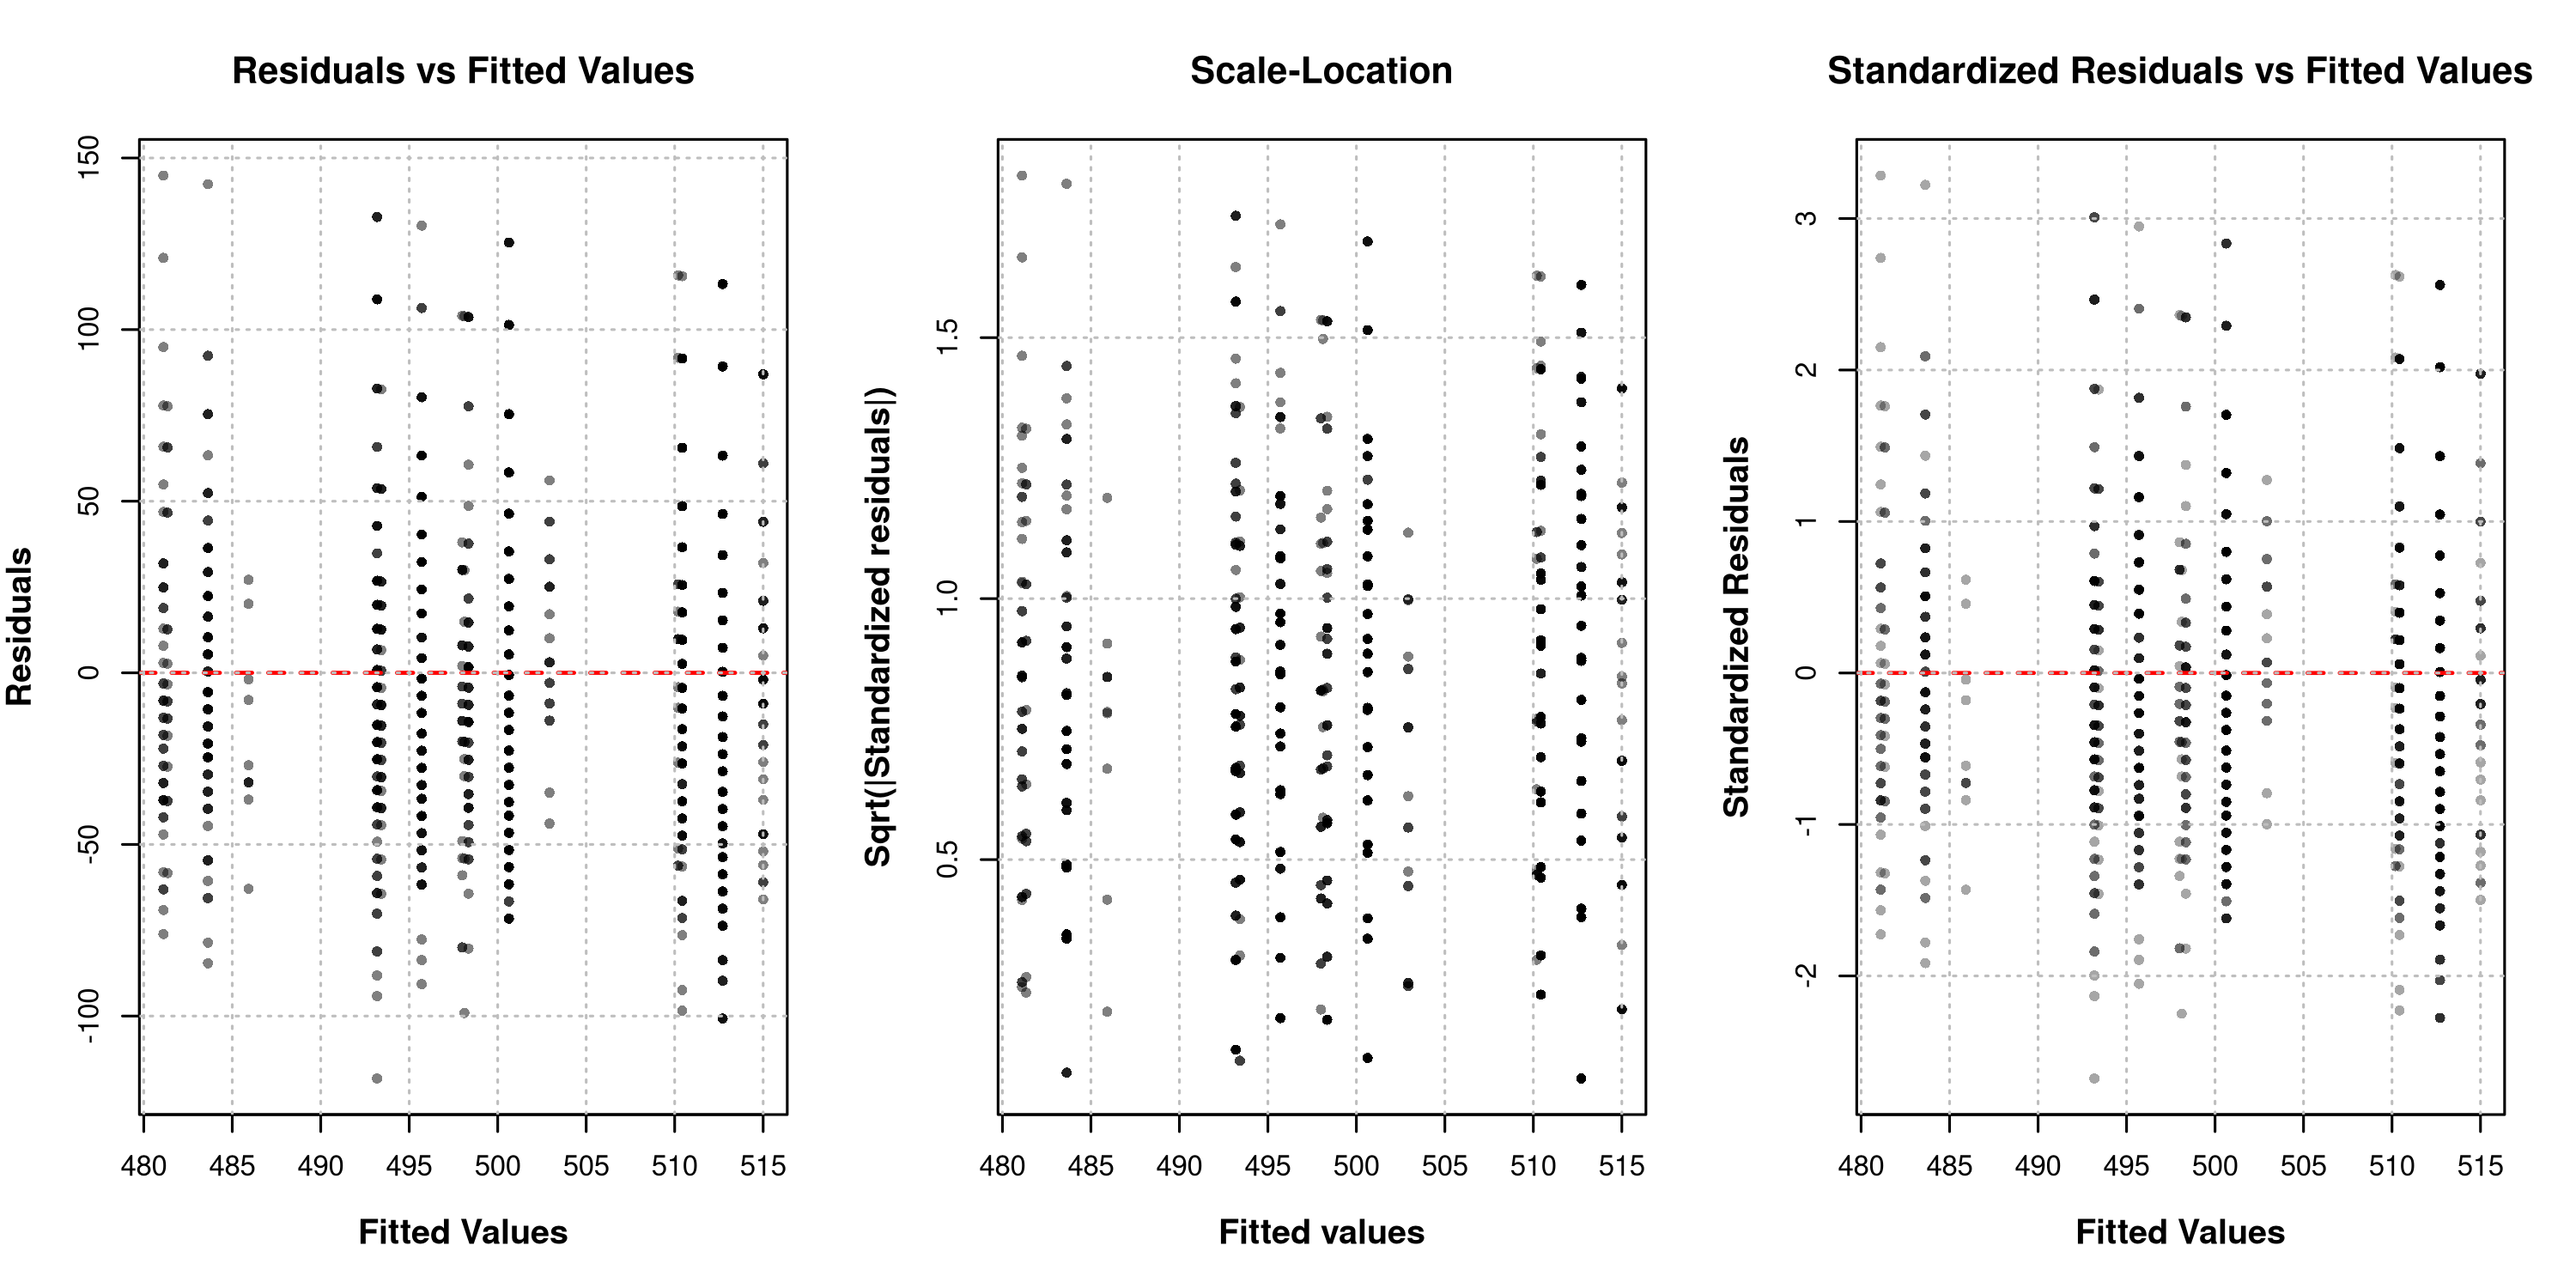
\includegraphics[width=0.7\textwidth]{img/sensitivity_analysis_q1_diag.png}
    \caption{Diagnostic plots for Model 1}
    \label{fig:sensitivity_analysis_q1_diag}
\end{figure}

The residual vs fitted value plot shows the residuals, $\hat{Y}_{ijkl} - \bar{Y}_{ijk\cdot}$, for each $(i, j, k)$. If the errors are homoscedastic, we should expect to see equal variance across all factor levels and therefore a roughly equal spread of data across all factor levels. In this case, for all but two factor levels, we observe the expected result. Note, however, that there are two factor levels with a considerably smaller range than the others. These smaller variance factor levels are associated with students in regular sized classrooms in urban schools who are receiving free lunch (fitted test scores of approximately 485.9) and students in regular sized classrooms in urban schools who are not receiving free lunch (fitted test scores of approximately 502.9). As seen in Section \ref{section:descriptive}, the urban schools were by far the least represented in the dataset, so the smaller perceived variance across these levels may be a bias due to missing data and not a true feature of the population. More target research would be needed to address this question.

The standardized residuals vs fitted values plot on the right of Figure \ref{fig:sensitivity_analysis_q1_diag} shows the standardized residuals\footnote{Here, $i$ indexes the data frame of values, not the factors}, $e_{i} / \sqrt{\mathrm{MSE}(1 - h_{ii})}$, vs the fitted values. This allows us to assess the existence of outliers in the dataset; if significant outliers are present, we would expect to see many standardized residuals exceed, say, three standard deviations from the mean. In the present case, we see a few falling outside of that region, but largely the data are as one would expect of a dataset without significant outliers. If the errors are truly $N(0, \sigma^2)$, then $\mathbb{P}(|X| > 3\sigma) \approx 0.27\%$ for any data point $X$. The number of points exceeding three standard deviations from the mean is larger than 0.27\% of the students in the study, which is a sign of possible outliers. Nonetheless, the data shows that the number of outliers is relatively small and with therefore be unlikely to have a significant impact on the analysis.

Figure \ref{fig:sensitivity_analysis_q1_errors} shows a histogram of the residuals across all factor levels.

\begin{figure}[H]
    \centering
    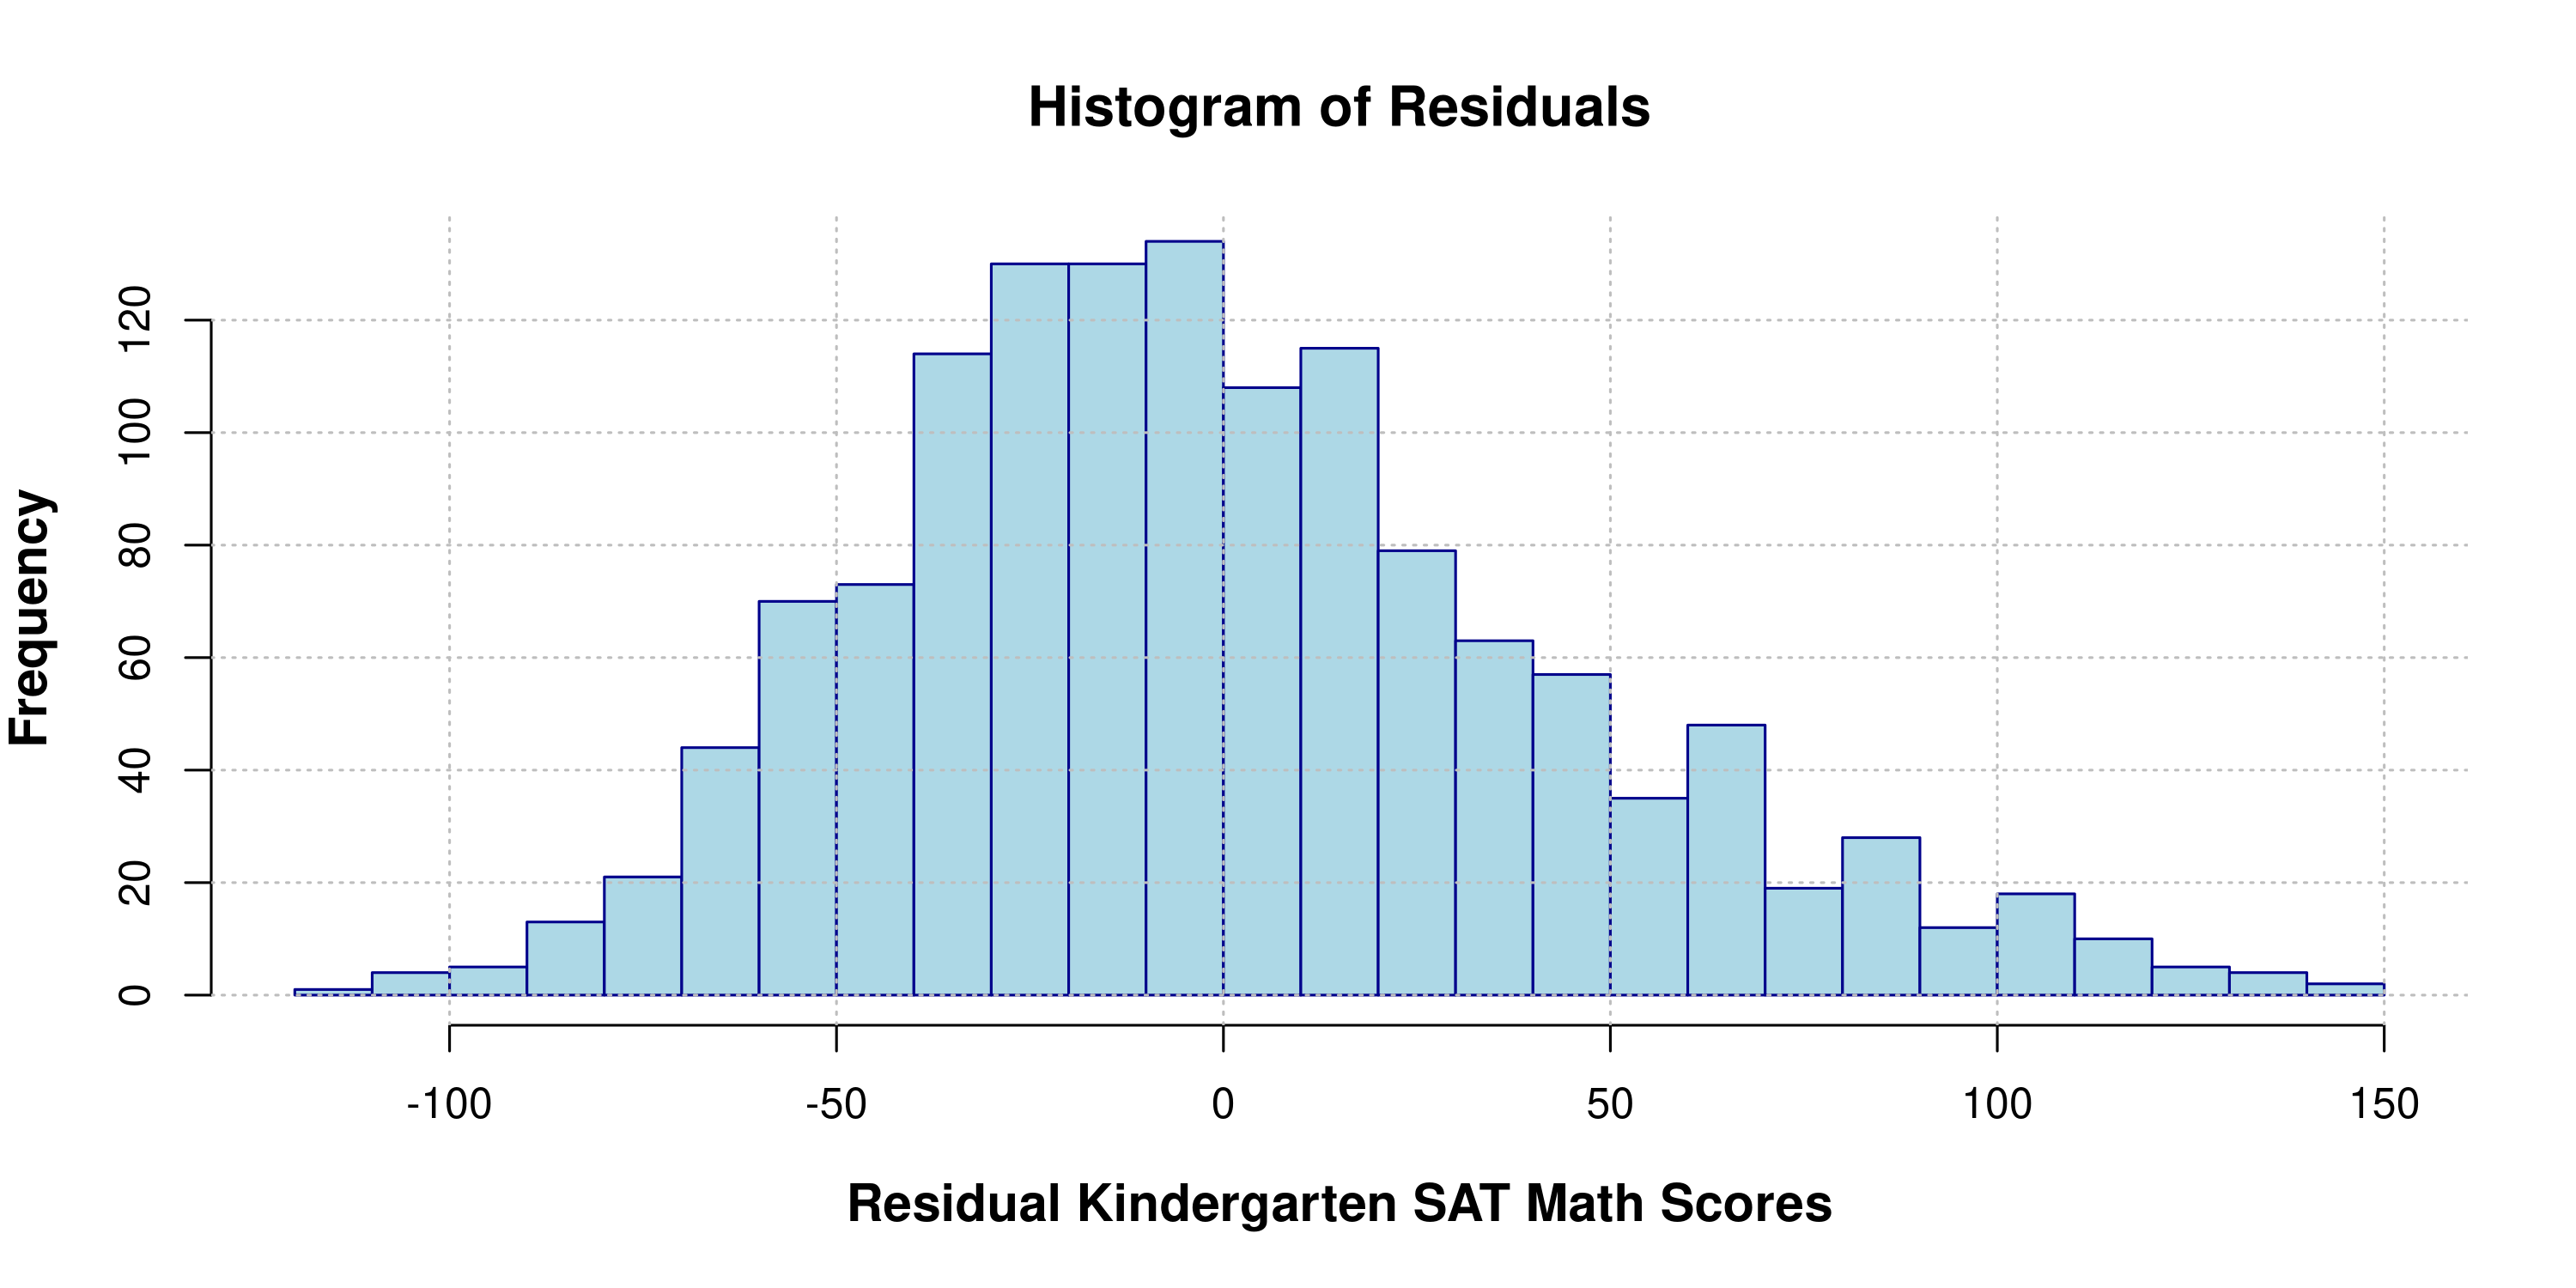
\includegraphics[width=0.7\textwidth]{img/sensitivity_analysis_q1_errors.png}
    \caption{Residual histogram for Model 1}
    \label{fig:sensitivity_analysis_q1_errors}
\end{figure}

This histogram reinforces the comments made above: the residuals appear to be roughly normal (and hence the errors may be normal as well), but the right tail is heavier than expected due to the presence of large outliers. To further examine the impact of outliers on our residuals, we plot the error distributions disaggregated by the relevant factor levels in our analysis in Figure \ref{fig:sensitivity_analysis_q1_box}.

\begin{figure}[H]
    \centering
    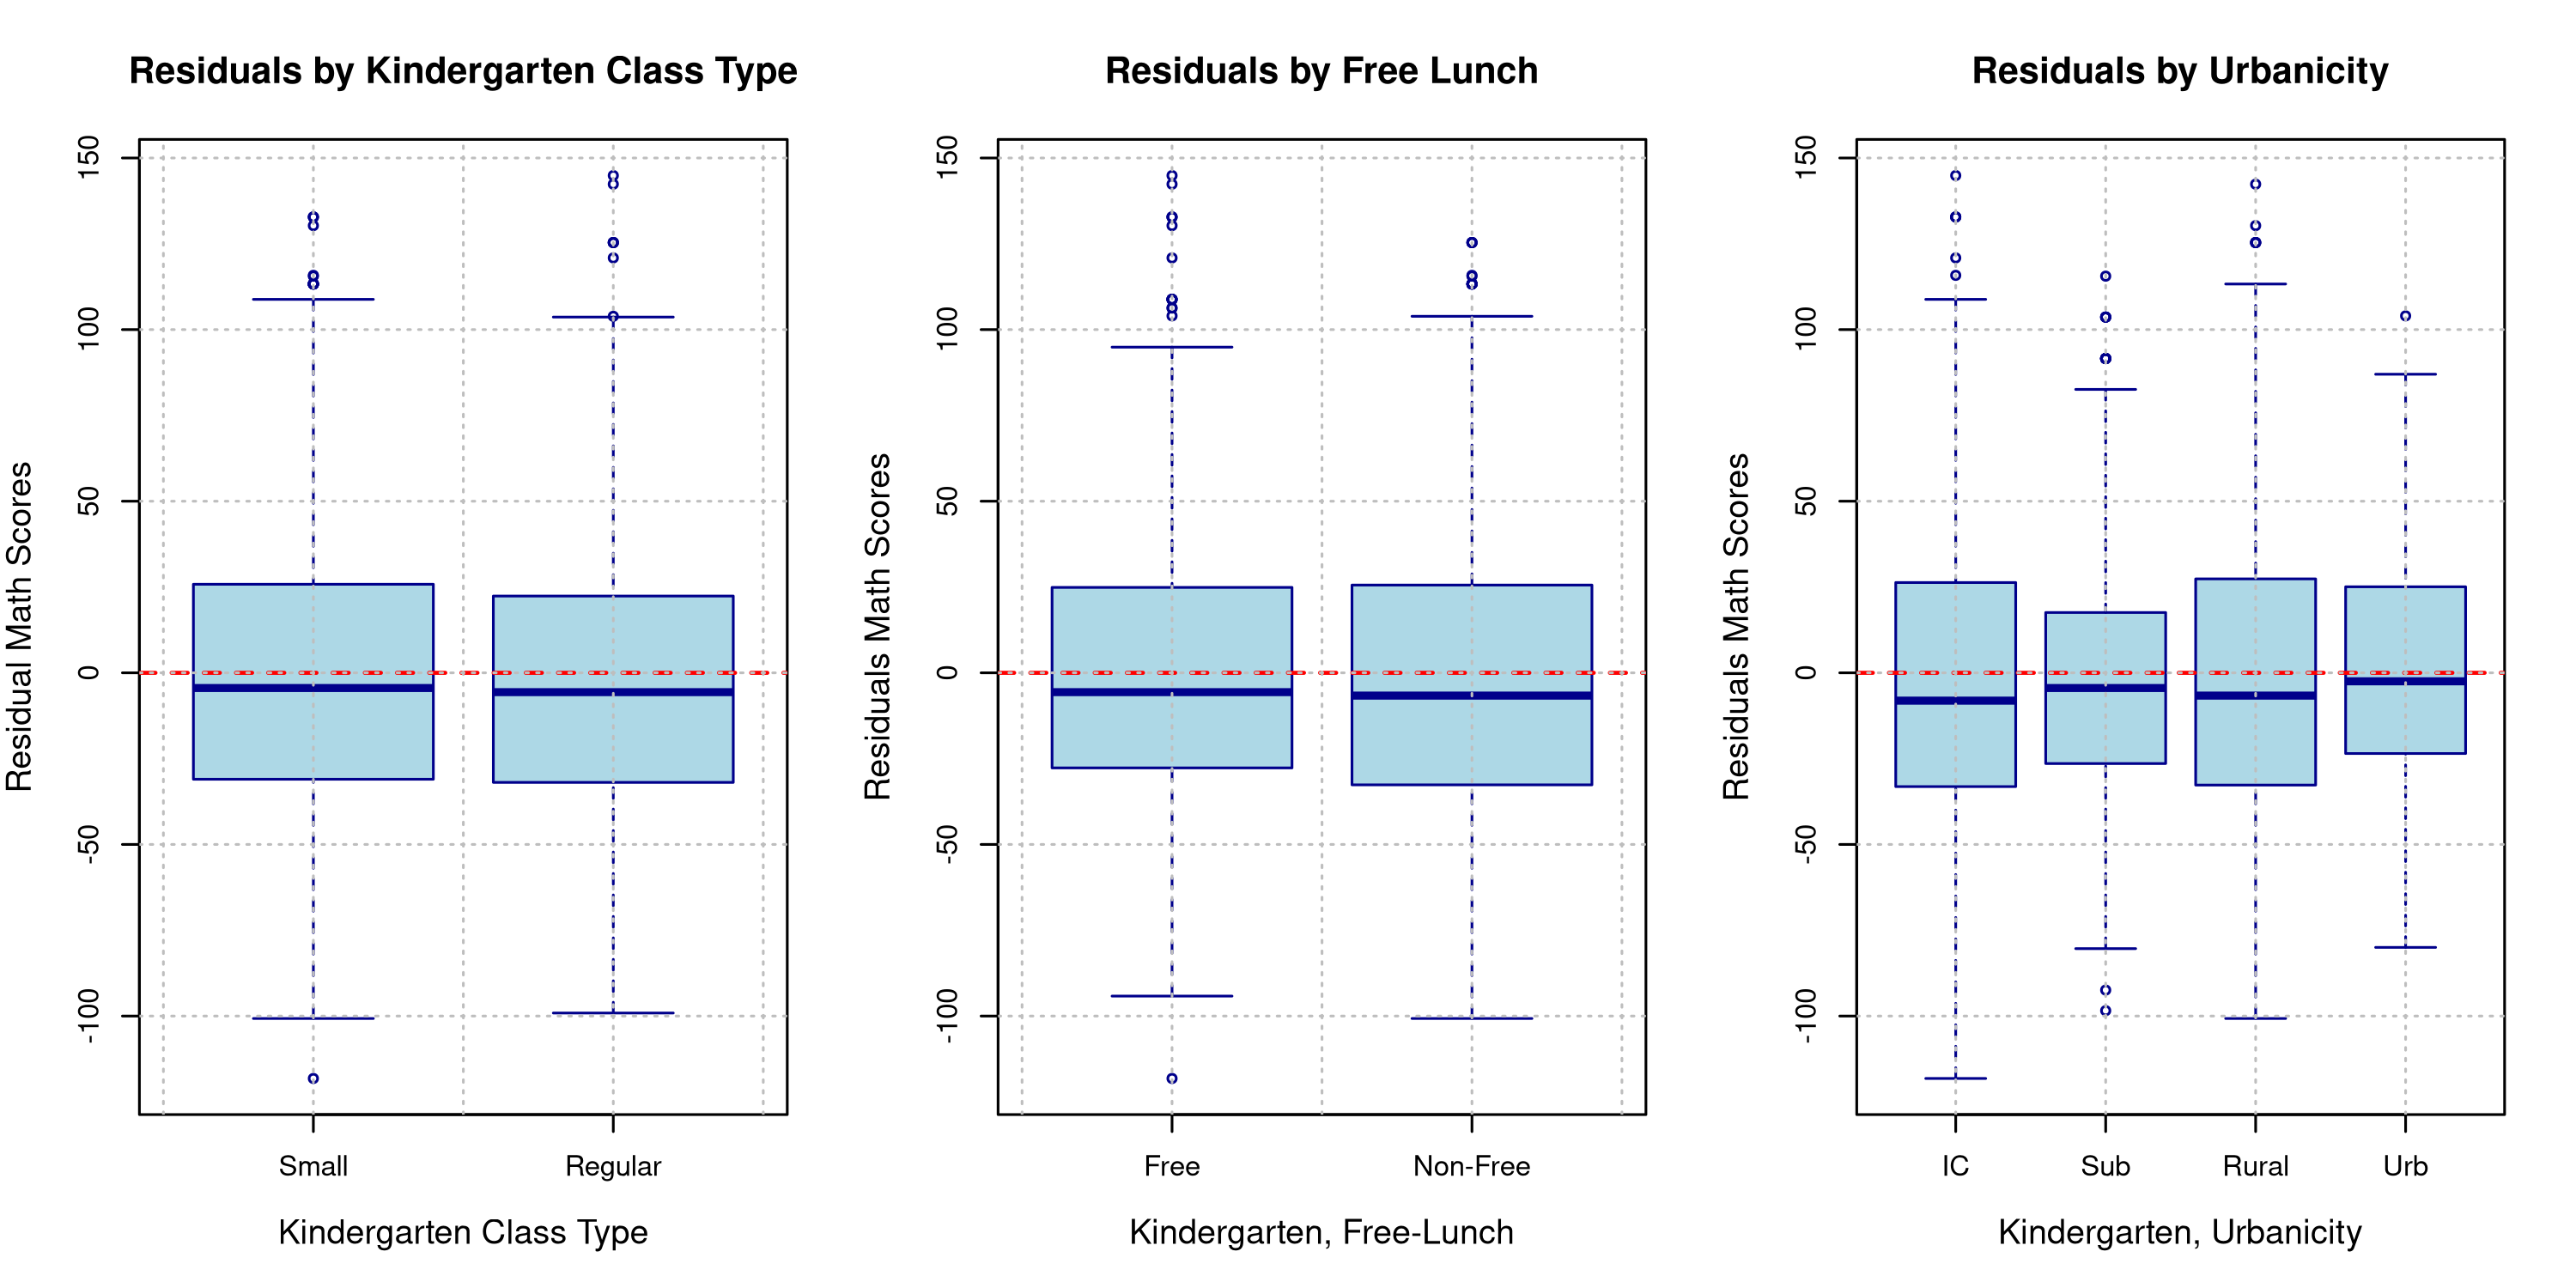
\includegraphics[width=0.7\textwidth]{img/sensitivity_analysis_q1_box.png}
    \caption{Residual boxplots by factor level for Model 1}
    \label{fig:sensitivity_analysis_q1_box}
\end{figure}

Again, outliers are present throughout all factors and all factor levels. They appear to be the most numerous among regularly sized classrooms than small classrooms, among students receiving free lunch than those that do not, and among inner city schools than those in other population densities.

In all, the assumptions of an ANOVA model are largely met, with the possible exception of outliers. A future analysis could be done to remove these outliers from the dataset entirely before fitting the model. 

\subsection{Mixed Effects Model Diagnostics}

For our mixed effects model which assesses if it is educationally advantageous to switch to smaller classes after being assigned to regular sized classes, it is important to analyze the model diagnostics to evaluate performance, detect potential confounding variables, and examine residual distributions. Given our response variable math scores is continuous, it is appropriate to use the common Pearson residual defined as $r_{ij}=\frac{Y_{ij}-\hat{Y}_{ij}}{SD(Y_{ij})}$, where $Y_{ij}$ is the observed value for row \textit{i} and column \textit{j}, $\hat{Y}_{ij}$ is the expected value, and $SD(Y_{ij})$ is the standard deviation. 

Ideally, our model will include all relevant covariates to explain as much information about the response as possible, in which case the residuals would follow a normal distribution with constant variance. This also follows from the assumptions of ANOVA stated in 5.1. First, we can examine the residuals vs. fitted plot, which shows the Pearson residuals against the predicted values $\hat{Y}_{ij}$. 

\begin{figure}[H]
    \centering
    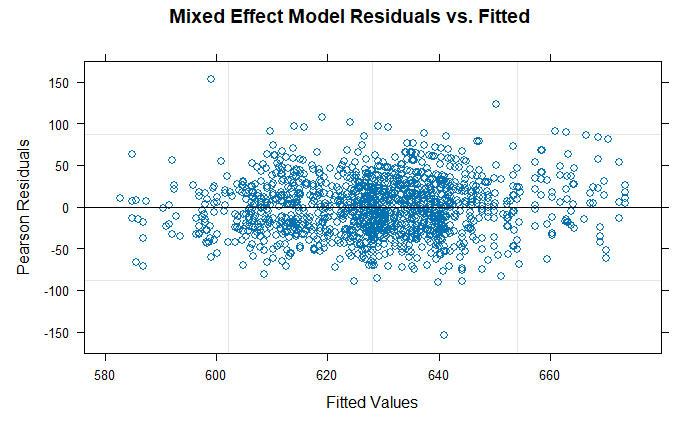
\includegraphics[width=0.7\textwidth]{img/sta_207_im1.png}
    \caption{Mixed Effect Model Residuals vs Fitted}
    \label{fig:sta_207_im1.png}
\end{figure}

The mixed effects residuals vs. fitted plot shows constant variance for all fitted values, which is reassuring that our model still predicts values well even at the high and low tails of the response variable distribution. It is also good to see that our residuals are centered around the 0, which validates the assumption 3 stated in section 5.1. Next, we can examine the distribution of the residuals, to ensure that the model predicts values well and therefore the error terms are best approximated by a normal distribution. 

\begin{figure}[H]
    \centering
    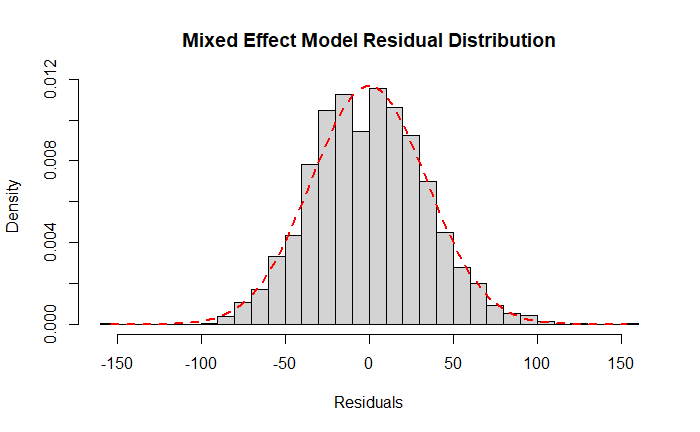
\includegraphics[width=0.7\textwidth]{img/sta_207_im2.png}
    \caption{Mixed Effect Model Residual Distribution}
    \label{fig:sta_207_im2.png}
\end{figure}

Our residual distribution displays a shape very closely related to the normal distribution. Another takeaway from this plot is that the tail approximations seem to be very good, as there is no strong skew on either side. This ensures that our model is accommodating for all possible sources of variation in math scores, and our selected covariates have predictive capability. Finally, to ensure there are no significant outliers in our dataset, we can observe the standardized Pearson residuals vs the student index. This will help us gauge how the model behaves for large residuals, or equivalently high observed values $\hat{Y}_{ij}$. 

\begin{figure}[H]
    \centering
    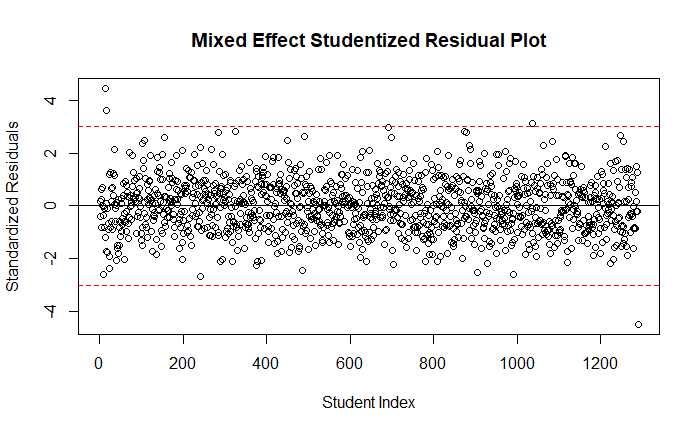
\includegraphics[width=0.7\textwidth]{img/sta_207_im3.png}
    \caption{Mixed Effect Model Studentized Residual Plot}
    \label{fig:sta_207_im3.png}
\end{figure}

The studentized residuals are defined as $r_{ij}=\frac{Y_{ij}-\hat{Y}_{ij}}{\hat{\sigma}\sqrt{1-h_{ij}}}$, where all other terms are defined as before, and $\hat{\sigma}$ is the estimated error variance. The red dotted lines three standard deviations away from the mean 0, to denote the bounds in which 99.7\% of the data should fall under. This also follows from the fact that the studentized Pearson residuals follow the standard normal distribution, mathematically put: $r_{ij} \sim N(0, 1)$. 

Our mixed effect studentized residual plot shows only 3 or 4 values outside the 3 standard deviation bounds, which denotes roughly 0.3\% of the data. This is to be expected as per the 68-95-99.7 rule of a normal distribution \cite{Michael2019_normal_dist}. 

In all, our covariates in the mixed effects model successfully captured all the necessary information in the response variable math scores. This is demonstrated by the residuals having normal distribution with mean 0 and variance $\sigma^2$, $r_{ij} \sim N(0, \sigma^2)$. The model does well at predicting values furthest away from the expected value, as determined by the tails having no strong skew. The studentized residual plot shows some values outside the three standard deviations away from the mean, however this is to be expected. 

\section{Conclusion}\par
\label{section:conclusion}

In conclusion, we sufficiently analyzed if smaller class sizes disproportionally benefit lower income students in early elementary school, and if it is educationally advantageous to switch to smaller class sizes after being in regular sized classes. Our analysis and dataset were supported by the STAR publication, Shizhe Chen's lecture notes, and other related literature. We opted to use math scores as the performance metric for students because we believe it captures all the meaningful insights needed to evaluate their academic standing. Low income status was determined by a students' participation in their schools' free lunch program, which may not be the best representative measure, however it is deemed appropriate for this analysis. We quantified switching to small classes as in any of the 4 years of school from kindergarten through third grade, if the student was assigned regular sized classes and at any point switched to small size classes. We chose to omit the students in the regular sized classes with aide entirely because we did not want to group with with regular sized classes because of confounding variable precaution, and sample size concerns. 

To begin our analysis, we further investigated the dataset by examining the distribution of school urbanicity (school location zone), the race proportions, and the number of schools by student income status. This information aided us in understanding the distribution and initial behavior of the covariates. It also helped us narrow down which predictors to include in which model. Next, we visualized the difference by grade of the math and reading scores between genders. This gave us appropriate understanding of the relationship between test scores by grade, along with how math and reading scores relate. We also examined the non-compliance observations, or students who opted out of the experiment to switch class sizes. We assumed this decision to be independent for modeling purposes. The non-compliers are important to analyze to assess if it is educationally advantageous to switch to smaller class sizes after being assigned to regular class sizes. 

To assess if smaller class sizes disproportionally benefit lower income students, we settled upon the three way anova model with response variable math score, and covariates class type, free lunch status, and school location (urbanicity). The F-test to detect if group means differ for each covariate group resulted in p-values much lower than our $\alpha=0.05$, signifying statistically different means in group class type and free lunch status. Contrary to our initial theory, urbanicity group means do not have significantly different math scores. 

To examine if it is educationally advantageous to switch to smaller class sizes after being assigned to regular class sizes, we can implement the mixed effects model with the random intercept term, trend denoting class size for each year, gender, race, free lunch status, and teacher years of experience. Table \ref{tab:mixed_results} outlines the results of our mixed effects model, with race, and free lunch status being the most significant covariates. We also calculated the Intraclass Correlation Coefficient, showing that 13.6\% of the proportion of variance is explained by difference between schools. 

We explored all statistical options needed to understand if smaller class sizes disproportionally effect lower income students, and if switching to smaller class sizes at any point in grades kindergarten through third grade is academically advantageous, determined by math score increases. We used appropriate models which explained variance well and resulted in significant covariates. We determined the important predictors by the F-test for difference of group means. Our analysis consisted of sufficient methods and we have reached a valid conclusion. 

\bibliographystyle{plain}
\bibliography{references}



\end{document}